%----------------------------------------------------------------------------
\chapter{\bevezetes}
%----------------------------------------------------------------------------

Due to the increasing complexity of embedded systems, and software systems in general, the design, implementation and analysis of these systems is getting more and more difficult on lower levels of abstraction, thus, the modeling of these systems should happen on a higher level. One feasible way to implement that is the so-called \textit{model-driven development} paradigm, which will be detailed later in this chapter (in the next section), along with a way to verify the correctness of these models through formal (verification) methods. This is the motivation of the framework deatiled in \cite{GammaVince2018}, to which a formally verifiable action language is going to be introduced.
%----------------------------------------------------------------------------
\section{Modeling and Verification of Systems} \label{mdsdForm_section}
%----------------------------------------------------------------------------
As a result of the application of the modeling concept in several (completely different) domains, first of all, we need to define the meaning of \textit{model} in this document.
\begin{definition}[Model]
	A model is the simplified image of an element of the real or a hypothetical world (the system), that replaces the the system in certain considerations. [REMO előadásból]
\end{definition}
Models can grasp various aspects of a system. Structural models describe the structure of the system, representing knowledge regarding the the parts of the system and the properties and connections of these parts. This means that the model describes static knowledge and not temporal change. On the other hand, behavioral models describe the change of the system over time through its changing of states and processes. Thus, these models represent dynamic knowledge about the system. These categories do not cover every aspect of the system, and usually cannot be separated this well in practice (practical applications). There are several possible formalisms for both kinds of models, which will be discussed in section 1.2 [REMO előadásból]

Model-driven software development (MDSD) is a software development methodology that utilizes domain models as the primary artifact throughout the entire software development process. This approach splits the traditional development into two parts. The first part is infrastructure development, during which the modeling language, platform and transformations are defined. The second part, application development, involves only modeling in the application domain. This strongly simplifies the design phase by efficient reuse of code and early validation. [MDSD előadásból] The major advantage of this methodology is the productivity improvement during the development of a (software) system, achieved through the fact that it is possible to derive different design artifacts, like documentation, source code, configuration and even other models from the system model.  \cite{RoadToModelTransf} One possible implementation of MDSD is the so-called Y-Model devleopment process [TODO cite] (see \refstruc{fig:yModel}).
\begin{figure}[!ht]
	\centering
	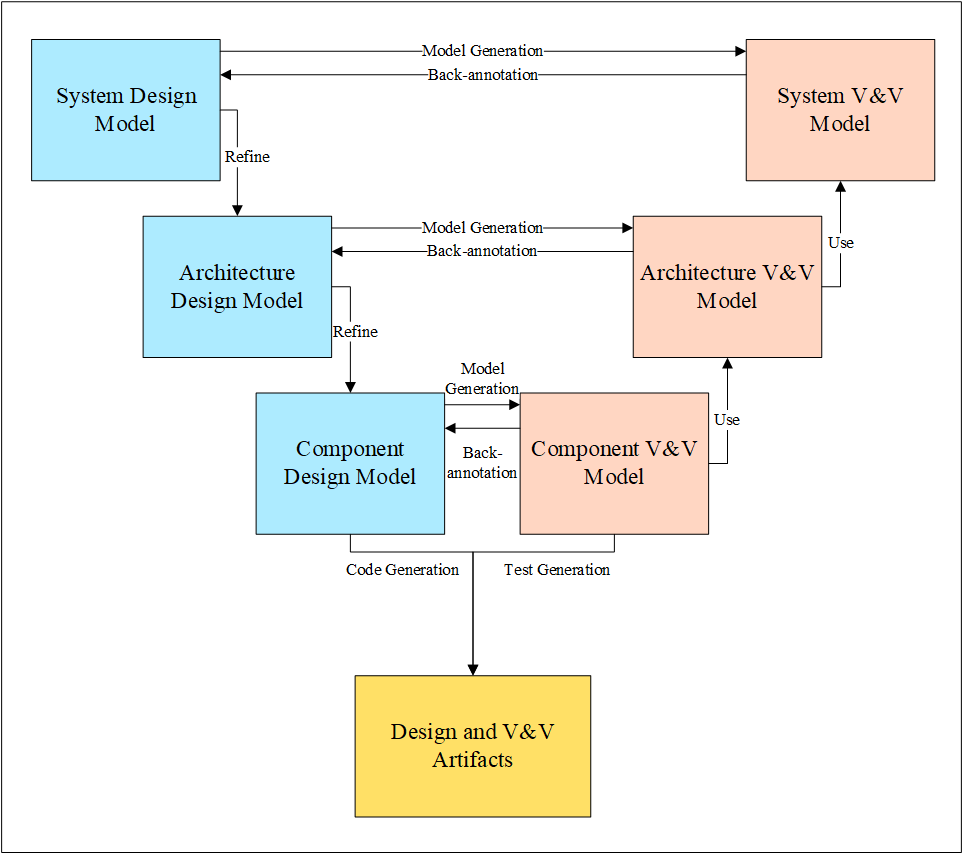
\includegraphics[width=70mm, keepaspectratio]{figures/yModel.png}
	\caption{The schematic description of the Y-Model}
	\label{fig:yModel}
\end{figure}

As the formal verification of the correct behavior is often a requirement against <fault tolerant> systems, this ability to transform the system (design) model into other models - in this case a verification model - proves to be a particularly useful quality. The precise formal analysis of these models either confirms the correctness of the given model, or provides the problem or problems where the model does not meet the requirements. These faults can then be back-annotated to the high-level models to allow system designer to make corrections, even in the early phases of the development process. \cite{RoadToModelTransf}

Formal verification is the act of comparing the design model of a given system against certain requirements formulated by the user. This process requires mathematically precise design models and requirement specifications, but guarantees mathematical precision in its result as a proof of correctness or counter-example of the correct behavior.
Model checking \cite{ModelCheckingClarkeGrumberg} is a formal verification technique for a finite-state model of a system, which explores the state-space of the given model soundly, exhaustively and automatically. This results in a complete analysis of the behavior of the given system unlike in case of simulation or testing, that only verify certain parts of it.

%----------------------------------------------------------------------------
\section{Different formalisms for modeling the behavior of systems} \label{modeling_section}
%----------------------------------------------------------------------------

Different kinds of behavioral models <grasp> different aspects of the modeled system. \textit{State-based models} focus on the current state of the system and its change of state in response to the events of its environment. The course (process) of this change is secondary, and these models consider these so-called transitions instantaneous. Examples of this kind of modeling include UML State Machines \cite{UMLStandard} or Statecharts \cite{HarelStatechart87}. On the other hand, \textit{process models} focus on the series of actions a system takes in order to achieve its goal, and these actions - called processes - possess a temporal <extent>. Examples of this kind of modeling include UML Activity Diagrams \cite{UMLStandard}, but the control flow of popular imperative programming languages (e.g. C/C++, Java) is also a process model[REMO előadásból].

For a model to be interpretable, executable or formally verifiable, it has to be given according to the predefined rules of model creation in the given domain. This set of rules is provided by modeling languages.
\begin{definition}[Modeling Language]
	A modeling language consists of the following elements:
	\begin{itemize}
		\item \emph{Metamodel:} a model defining the building blocks of the modeling language as well
		as their relationships.
		\item \emph{Concrete syntax:} a set of rules defining a graphical or textual notation for the
		element and connection types defined in the metamodel.
		\item \emph{Well-formedness constraints:} a set of constraints that models have to meet in order
		to be deemed valid in the modeling language.
		\item \emph{Semantics:} a set of rules that define the meaning of the element and connection
		types defined in the metamodel. Semantics can be either \textit{operational} (what should happen during execution) or \textit{denotational} (given by translating concepts in a modeling language to another modeling language with a well-defined semantics). [FORM]
	\end{itemize}
\end{definition}

If a part of the modeling language is missing or not precise enough - which is often the case for modeling languages used in engineering - an association must be made between the given model and a formal mathematical model. Process models, thus imperative programming languages can be easily transformed into Turing machines and state-based models correspond well to finite state machines[REF?]. One of the most important questions in the verification of computer programs is the ability to decide the termination of the given program, as to prove its correctness, the model checker must traverse each possible execution of it. This problem is known as the \textit{halting problem} and it is proven in \cite{Turing1936} that in general, it is not possible to solve for all program-input pairs. However, for finite state machines the problem is solvable \cite{Minsky:1967}, and this is one of the reasons, why state-based models are the common way of modeling when designing safety critical systems, even if they possess less expressive power than other kinds of automata. 

\begin{figure}[!ht]
	\centering
	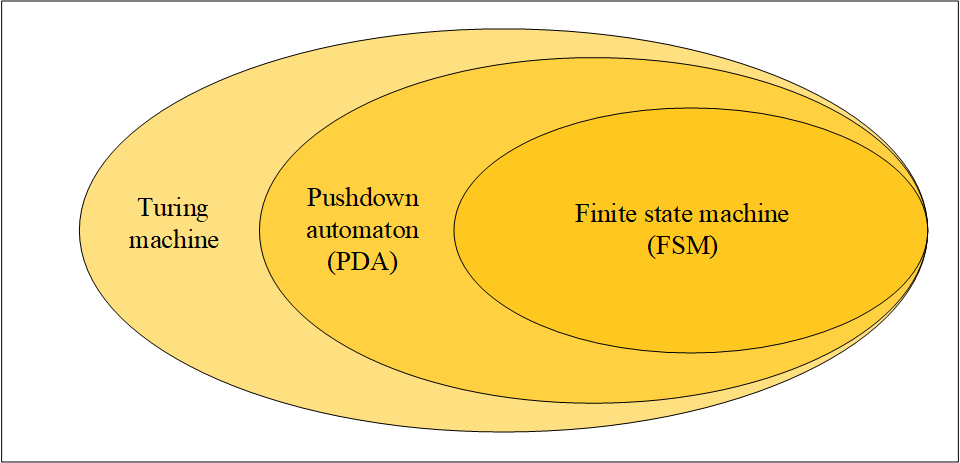
\includegraphics[width=100mm, keepaspectratio]{figures/automataTheory.png}
	\caption{Classes of automata}
	\label{fig:automataTheory}
\end{figure}

%----------------------------------------------------------------------------
\section{Overview} \label{Overview_section}
%----------------------------------------------------------------------------
To describe the reactions of to the events of the outside world in state-based models, an action language that describes the process of the reaction of the system is required. The language should be able to describe the <expected> behavior of embedded systems but it should also be formally verifiable. Naturally, it cannot be a turing-complete language, as the termination of such programs is undecidable. In the following chapters, one possible implementation of a language is going to be detailed. This language supports control structures of high-level general-purpose programming languages (e.g. foreach-loop) and the correctness or incorrectness of the program implemented in it is also decidable. 

Chapter 3 [TODO REF] deals with the background of the work. Precise definitions are given for the relevant formalisms as well as the corresponding formal verification techniques. Then, action languages of existing tools are analyzed with special regard to their expressive power and verification possibilities. Also, a brief summary of the target frameworks is given.[Gamma-Theta]
In chapter 4 [TODO REF] the above mentioned action language is going to be detailed. First of all, the syntax and planned semantics of the language elements, then the validation rules that (...). After that, the transformation of the AST into various models is going to be detailed, with special attention to the execution and verification of the model.
Chapter 5 [TODO REF] gives a brief summary of the applied technologies, respectively: EMF, Xtext, Xtend, VIATRA.
Chapter 6 [TODO REF] gives a case study for the application of the described language. Lastly, the correctness of each of the language elements is going to be validated.